\section{Introduction}

% \blue{
Learning a robust and generalizable policy for robotic manipulation through policy learning has long been a challenging problem~\cite{kim2020domain}, with traditional reinforcement learning approaches \cite{choi2024domain,bica2021invariant} often suffering from poor robustness and limited generalization. Recently, the rapid advancement of foundational Vision-Language Models (VLMs) \cite{awadalla2023openflamingo,liu2024visual} has demonstrated remarkable capabilities in multimodal understanding and generalization. Leveraging large-scale real-world robotic datasets \cite{o2024open,fang2024rh20t}, pioneering works \cite{zitkovich2023rt,octo_2023,niu2024llarva,kim24openvla} have introduced Vision-Language-Action (VLA) models, which integrate vision and language modalities to directly generate robotic actions in an end-to-end manner. This emerging paradigm holds great promise for enhancing the adaptability and generalization of robotic control systems, but leaves a large computational demand.

To mitigate the extensive cost of VLA models, existing works often adopt generic acceleration techniques, such as model lightweighting \cite{wen2024tinyvla}, quantization \cite{park2024quantization}, and early-exit \cite{DeeR-VLA}. While effective to some extent, these methods often require architectural modifications or retraining, and more importantly, they \textit{lack task-specific design tailored to the intrinsic characteristics of VLA tasks}. As a result, they struggle to achieve an optimal balance between inference speed and action accuracy.
% However, these approaches still involve substantial model parameters and often require architectural modifications or retraining, limiting their generalizability and applicability to off-the-shelf VLA models.
In this paper, we step into the nature of VLA robotic manipulation that is intrinsically different from the VLM models. Specifically, VLA tasks involve sequentially processing a stream of temporally adjacent visual observations, where the environment often exhibits high spatial redundancy across time. As shown in Figure~\ref{fig:motivation}, large portions of the visual scene, especially background regions, remain static and semantically irrelevant to action decisions, yet are processed repeatedly at each time step. These static tokens contribute significantly to computational overhead while providing limited utility for downstream control. This motivates our proposed token caching mechanism, which explicitly exploits temporal redundancy in visual inputs to reduce redundant computation without compromising decision quality.

\begin{wrapfigure}{r}{0.57\textwidth}
    \centering
    \vskip -0.15in
    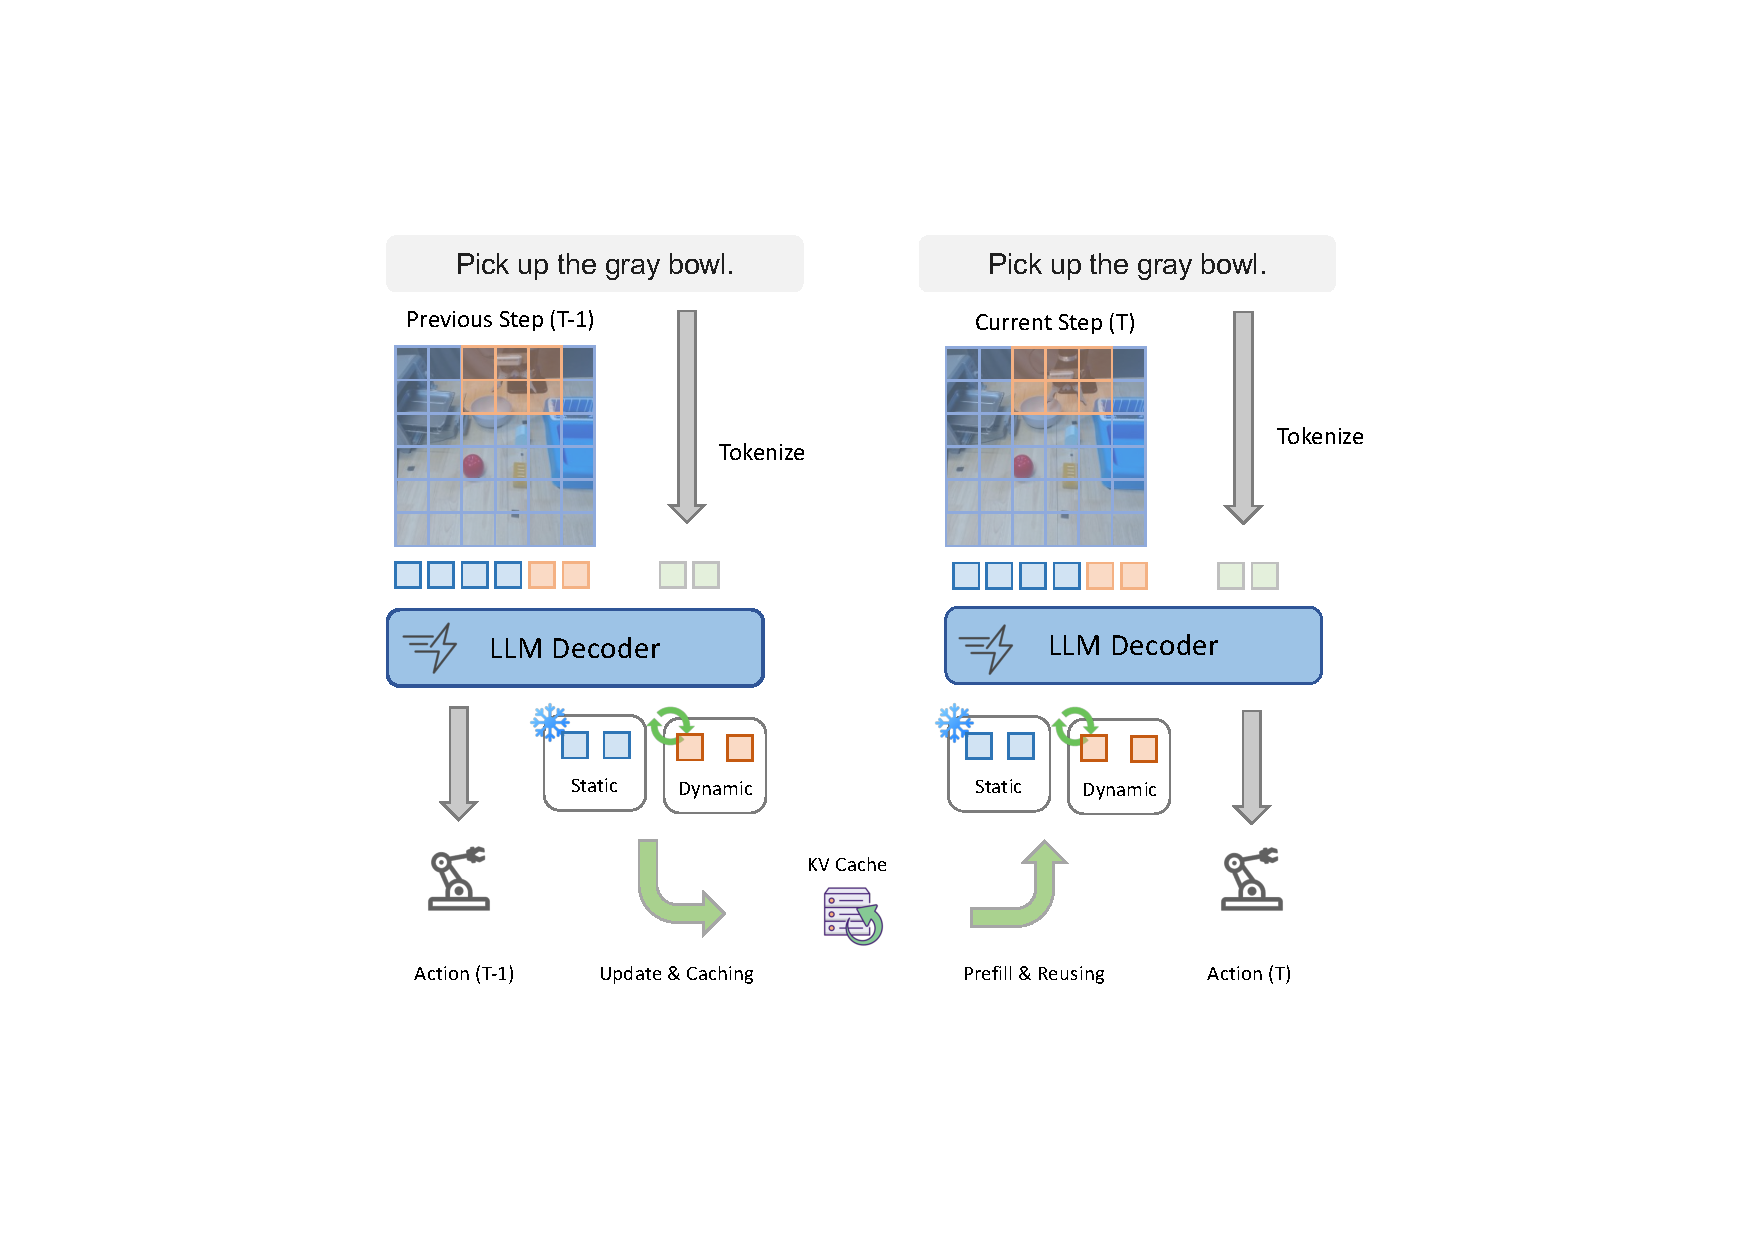
\includegraphics[width=3.1in]{fig/motivation.pdf}
    % 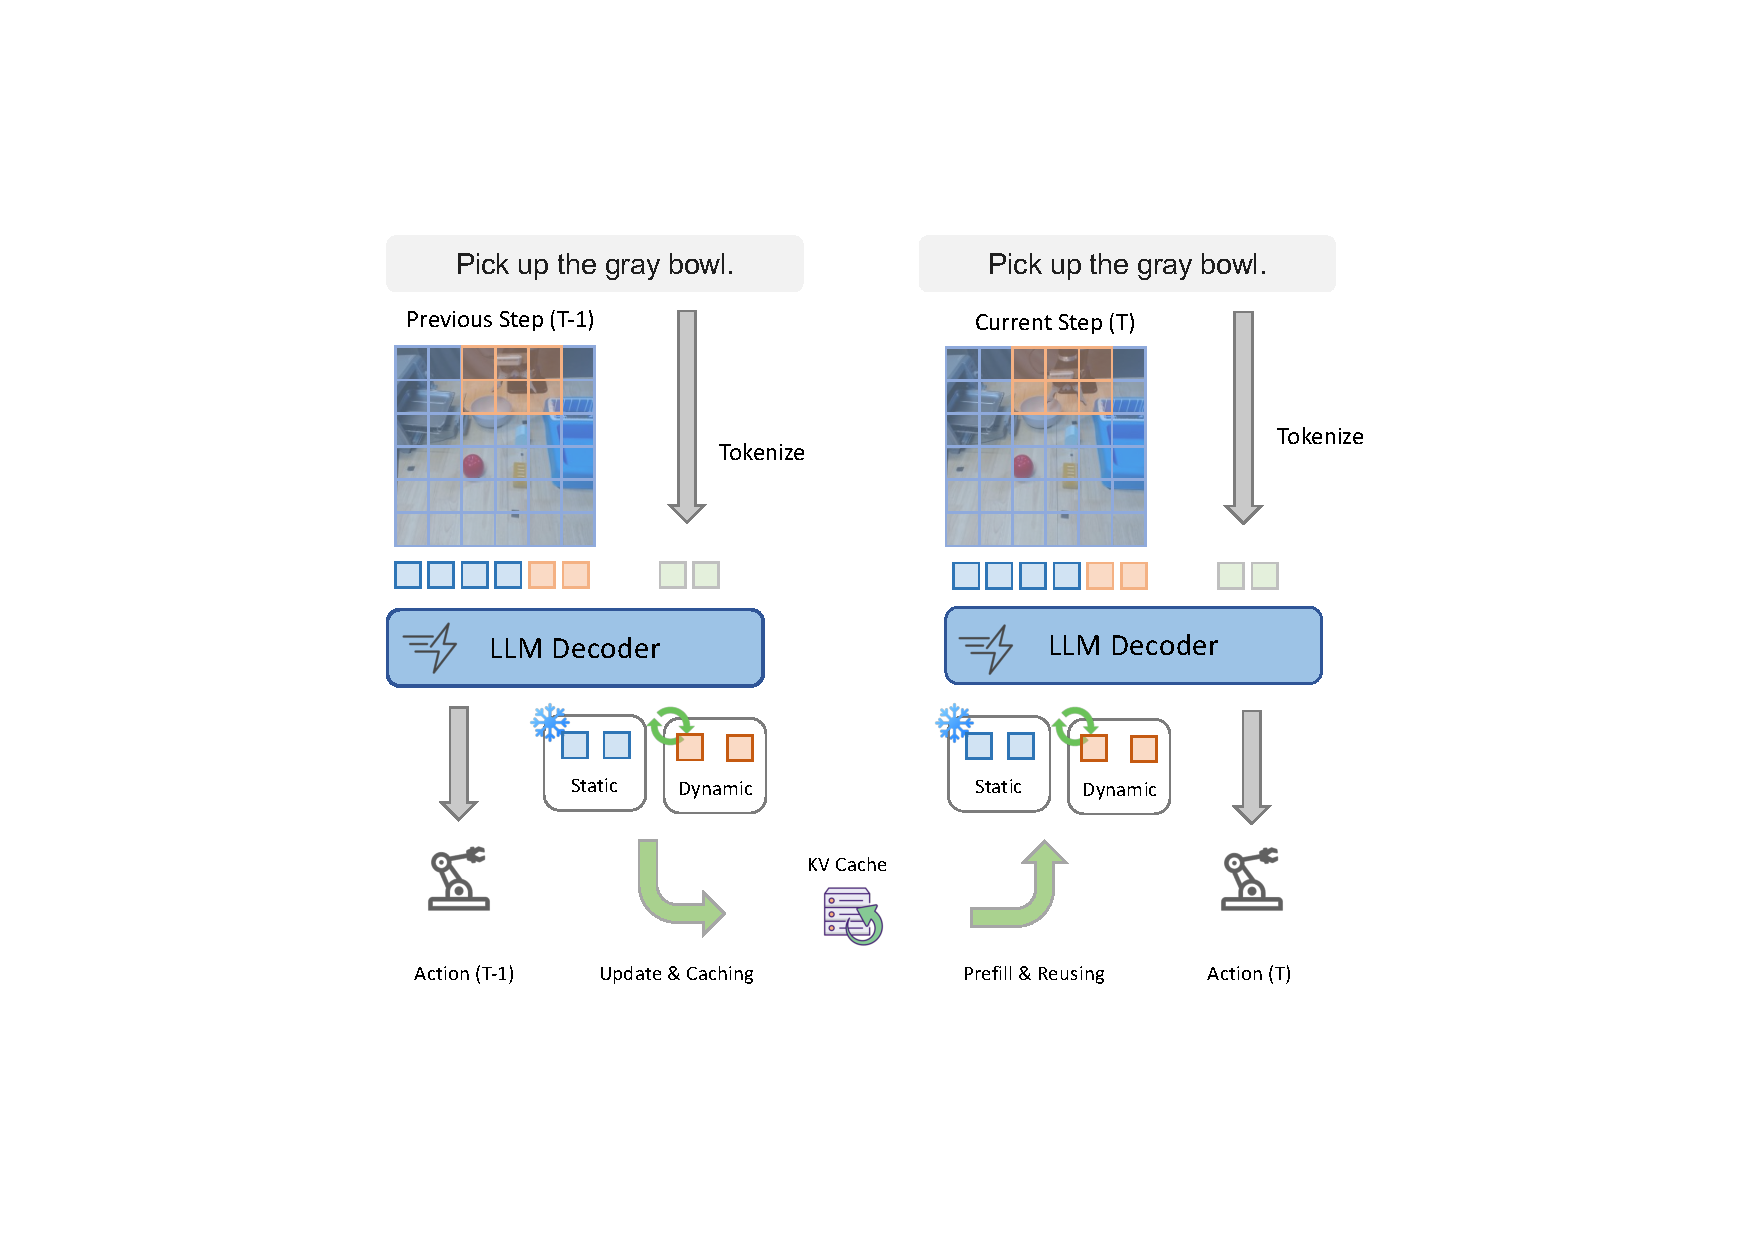
\includegraphics[width=2.95in]{fig/motivation.png}
    \vskip -0.05 in
    \caption{During the inference of the VLA model, static tokens of the input image remain largely consistent across steps. This consistency allows for caching the computations of these tokens from the previous step.}
    \vskip -0.1in
    \label{fig:motivation}
\end{wrapfigure}

To address the inefficiency introduced by repeatedly processing static visual information, we present \textbf{VLA-Cache}, a training-free inference acceleration method that exploits temporal continuity in robotic perception. Rather than recomputing all vision tokens at every timestep, VLA-Cache identifies tokens that exhibit minimal change between adjacent frames and reuses their cached key-value (KV) representations to bypass redundant computation. However, we observe that not all visually static tokens can be safely reused. Some tokens, such as those near the gripper or target object, may appear visually unchanged but remain semantically active and crucial for accurate action generation. Naively reusing all static tokens results in a significant performance drop as shown in Table ~\ref{tab:selection_ablation_inline}. To mitigate this, VLA-Cache incorporates a lightweight filtering mechanism based on decoder attention scores to exclude task-relevant tokens from reuse, ensuring that semantically critical regions are always recomputed with up-to-date features. Moreover, we observe that attention patterns vary across decoder layers, with deeper layers exhibiting more concentrated focus. To further optimize reuse, VLA-Cache employs a layer-adaptive caching strategy that dynamically adjusts the reuse ratio per layer based on attention entropy, prioritizing precise updates in sensitive regions. These two mechanisms together enable substantial reduction in decoding overhead, especially in large-scale language decoders (\textit{e.g.}, LLaMA~\cite{touvron2023llama}, Gemma~\cite{team2024gemma}), which typically dominate the compute cost in VLA systems.


The resulting method \textbf{VLA-Cache} offers a training-free and plug-and-play solution for accelerating VLA models without sacrificing action performance.  We evaluate VLA-Cache on robotic manipulation tasks across two simulated environments (LIBERO~\cite{liu2024libero} and SIMPLER~\cite{li2024evaluating}) and three state-of-the-art VLA models (OpenVLA~\cite{kim24openvla}, CogAct~\cite{li2024cogact}, and OpenVLA-OFT~\cite{kim2025fine}). VLA-Cache consistently delivers over \textbf{1.7$\times$ acceleration} with only minor drops in task success rate. Furthermore, we demonstrate its real-world applicability by deploying it on a \textit{Kinova Jaco2 robot arm}, achieving practical speedup under real-time control scenarios.
